% last-modified: 08.08.2024
% how-to-reproduce: /src/db-controller/notebooks/traceroute.ipynb

\section{Traceroute Analysis} \label{sec:traceroute-analysis}

Looking at traceroute results, we can make conclusions about the routing behavior of Starlink network devices. In the data we gathered more than forty million traceroute measurements. Those include primarily built-in measurements from RIPE Atlas probes to \textit{*.root-servers.net} for Starlink probes (\ac{ASN} 14593).

\subsection*{Routing Behavior}

\begin{figure}
	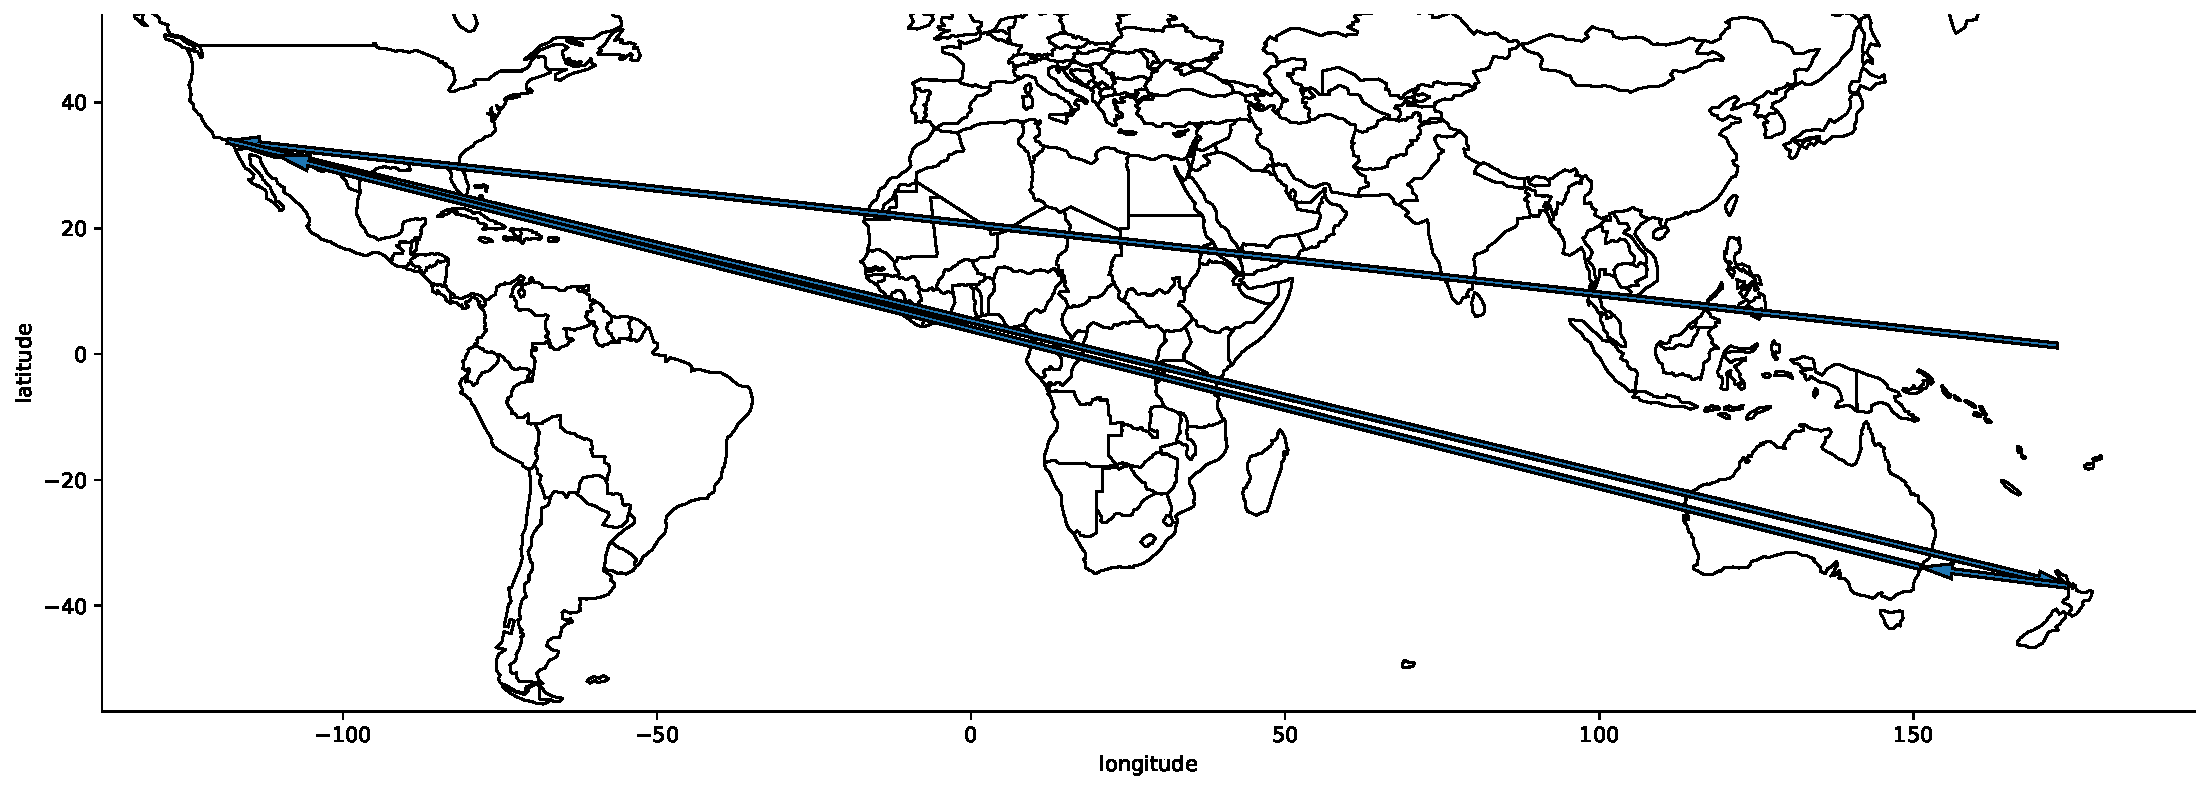
\includegraphics[width=\textwidth]{chapters/img/kiribati-example-traceroute.pdf}
	\caption{Visualization of a Traceroute from Kiribati}
	\label{fig:kiribati-example-traceroute}
\end{figure}

First, we found that the satellite hops are likely invisible to the traceroute. We conclude that as there are no hops visible above water, even for probes located in remote regions, e.g., Kiribati in the Pacific Ocean. In Figure~\ref{fig:kiribati-example-traceroute}, one can see a visualization of a traceroute result from Kiribati to \textit{f.root-servers.net}. One can see that the first visible hop is located in New~Zealand or an island to the north of New~Zealand. However, if satellites were visible, we'd be able to observe more satellites.

% TODO: Cite the statement that 4000km is too large for a single satellite. Everybody would ask here now: "But how much can they actually cover?"
Coming from the first insight, we can also conclude that \ac{ISLs} are enabled. If they were not, we would likely not be able to see a successful traceroute from Kiribati to a location. The next closest known \ac{PoP} is on Hawaii. However, the distance between both is 4000~km, which is more than a single satellite can cover. Aside from that, we do not observe the usage of the \ac{PoP} in Hawaii, but in more distant locations, which just strengthens the argument. Therefore, we conclude that \ac{ISLs} are enabled. This is special interest, as it was not clear in recent research \cite{Hauri2020}.

\subsection{Privacy Concerns in Traceroute Data}

One of the most important responsibilities of an \ac{ISP} is to ensure the privacy of its users. This also includes to route traffic only in trusted countries. In the case of Starlink, we were able to observe a different behavior. We looked at a slice of the built-in traceroute measurements from German Starlink probes and analyzed their most common targets. We filtered for anycasted servers (e.g., *.root-servers.net) and bogon IPs (i.e., IPs that cannot be associated with metadata).

% Input IP Hitlist
\begin{table}
	\caption{IP Hitlist for Built-In Traceroute Measurements}
	\label{fig:ip-hitlist-traceroute}
	\begin{tabular}{rllll}
		\toprule
		Hits  & City              & Country       & Organization & IP Address      \\
		\midrule
		10634 & Frankfurt am Main & Germany       & AS1299       & 62.115.37.20    \\
		8202  & Offenbach         & Germany       & Unknown      & 80.81.192.154   \\
		6207  & Amsterdam         & Netherlands   & Unknown      & 193.239.116.217 \\
		5582  & Frankfurt am Main & Germany       & AS2914       & 213.198.72.18   \\
		5257  & Frankfurt am Main & Germany       & AS3257       & 89.149.137.14   \\
		4932  & Chicago           & United States & AS14593      & 206.224.65.178  \\
		4916  & Chicago           & United States & AS14593      & 206.224.65.180  \\
		4850  & Chicago           & United States & AS14593      & 206.224.65.182  \\
		4755  & Chicago           & United States & AS14593      & 206.224.65.184  \\
		4358  & Miami             & United States & AS49791      & 81.31.213.126   \\
		4333  & Zürich            & Switzerland   & Unknown      & 185.1.147.30    \\
		4256  & Tokyo             & Japan         & Unknown      & 210.173.176.242 \\
		4179  & Chicago           & United States & AS14593      & 206.224.65.186  \\
		4035  & Chicago           & United States & AS14593      & 206.224.65.192  \\
		4014  & Frankfurt am Main & Germany       & AS6762       & 213.144.184.30  \\
		4010  & Chicago           & United States & AS14593      & 206.224.65.190  \\
		4005  & Chicago           & United States & AS14593      & 206.224.65.188  \\
		4002  & Frankfurt am Main & Germany       & AS1299       & 62.115.124.118  \\
		3990  & Singapore         & Singapore     & AS2497       & 202.232.1.69    \\
		3827  & Frankfurt am Main & Germany       & AS6939       & 72.52.92.70     \\
		\bottomrule
	\end{tabular}
\end{table}


In Table~\ref{fig:ip-hitlist-traceroute}, the top twenty most frequent hits of IP addresses are shown. The IP addresses are joined with data from IPInfo. As traffic goes from a German probe to an anycasted server, located in Germany, one would expect little traffic outside Germany, and none outside Europe. The top five IP addresses are located within or close to Germany, but the next five already involve traffic to the United~States. Here, we observe an unexpected behavior. Assuming that the data is not flawed, this is a clear violation of guiding privacy principles.

